\section{Results and Discussion}\label{sec:results-and-discussion}
Fig.~\ref{fig:schematic} was realized with damping factor $\zeta = 0.1$.
Using \eqref{eqn:damping}, $R_a = \SI{70.2}{\kilo\ohm}$.
The opamp supply power was set at \SI{+-15}{\volt}.
An input signal of 0.1\si{\voltpp} at \SI{50}{\hertz} square wave was applied to the circuit.
One pulse of the square wave will behave locally like a unit step function.

The output of this circuit is shown in Fig.~\ref{fig:overshoot}.
The large overshoot corresponds to significant underdamping, which is consistent with $\zeta = 0.1$.

\pagebreak

\begin{figure}[tbph]
	\centering
	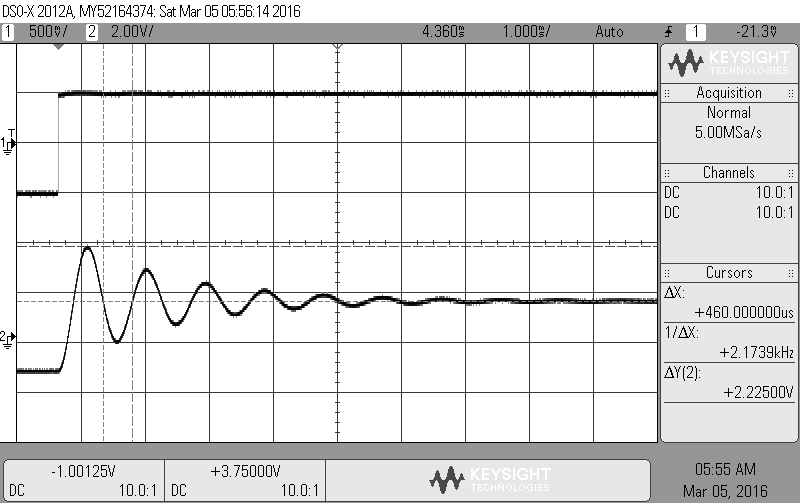
\includegraphics[width=0.7\linewidth]{graphics/overshoot}
	\caption{Measured response of second order system}
	\label{fig:overshoot}
\end{figure}

The measured values are $O_v = \SI{2.225}{\volt}$ and $T_p = \SI{460}{\micro\second}$.
As the transient response is damped, the value of the output settles to \SI{2.8}{\volt}.
This is consistent with $G = 1.8$.

Using equation \eqref{eqn:overshoot} and Fig.~\ref{fig:overshoot}, Zeta could be solved for. 
\begin{equation}\label{eqn:solveforzeta}
	{\ln(O_v) \over \pi} = {\zeta \over \sqrt{1 - \zeta^2}}
\end{equation}
The experimentally determined value of $\zeta$ was found to be $\zeta = 0.2467$.
Next, $\omega_0$ was solved for by rearranging \eqref{eqn:period}.
\begin{equation}\label{eqn:solveforomega}
	\omega_0 = { \pi \over T_p\beta }.
\end{equation} 
Solving equation \eqref{eqn:solveforomega} gives an angular velocity of $\omega_0 = 7048$.

Using the determined values for \zeta and \omega_0, a simulated time domain response was generated in matlab.